%% Status: 2015-12-30 Some parts collected from wiki.
%% TODO: Describe StellariumScope plugin

\chapter{Stellarium at the Telescope}
\label{ch:atTheTelescope}

Two plugins are bundled with Stellarium which are designed to be used
at the telescope: Oculars, which provides field of view hints for
telescopes, oculars and sensors, and TelescopeControl, which allows
you to send GOTO commands to many motorized telescopes. Other goto
telescopes are supported by an external plugin which you must install
separately: StellariumScope (section~\ref{sec:plugins:StellariumScope}). 

\section{Oculars Plugin}
\label{sec:plugins:Oculars}

This places a window on the screen that corresponds to the view
through a telescope or on a camera. It reads from an editable data
base.

When this plug in is active a circular view will appear around the
selected object depicting what would be seen by the viewing object. On
the top right hand side of the screen a menu will appear that can be
used to select the viewing device, e.g., Camera, Eyepiece, Barlow type
lenses, etc. This menu is filled with items from the \file{ocular.ini}
file in the \file{modules/oculars} folder. This file can be edited
from the Plugin's menu screen or with a text editor.

%TODO: Details?

\section{TelescopeControl Plugin}
\label{sec:plugins:TelescopeControl}

Stellarium has a simple control mechanism for motorised telescope
mounts. The user selects an object (i.e. by clicking on something -- a
planet, a star etc.) and presses the telescope go-to key 
%(see section \ref{sec:plugins:telescopeControl:goto})  <<<<<<<<<<<<<<<<<< YES, WHERE?
and the telescope will be guided to the object.

Multiple telescopes may be controlled simultaneously. 

%TODO Details?

The control interface uses the Meade or the Celestron protocol and
most telescopes use either one or the other so many different brands
of telescopes can be controlled. There is a third party Telescope
control system going under the name of ASCOM. They provide an
interface to stellarium and then translate the control into many other
forms (see section~\ref{sec:plugins:StellariumScope}).


\paragraph{WARNING}: \emph{Stellarium will not prevent your telescope from being pointed at the Sun. It is up to you to ensure proper filtering and safety measures are applied!}

\section{StellariumScope plugin}
\label{sec:plugins:StellariumScope}
StellariumScope is a free add-on that enables you to control your telescope with Stellarium. 

\paragraph{Features}
\begin{itemize}
\item Provides an interface between Stellarium and the ASCOM telescope drivers.
\item Provides the ability to both ``Sync'' and ``Slew'' the
  telescope. It's also possible to issue a stop/cancel command from
  Stellarium.
\item You can easily host Stellarium on one computer linked to another
  control computer that hosts the telescope driver.
\item The installation program will automatically install the
  documentation, but the link to the documentation is provided
  here\footnote{WHERE?} so you can read it before installation.
\item There are earlier releases still available on the downloads page on
  Welsh Dragon Computing site.
\end{itemize}

The original StellariumScope program was designed and implemented by
Scott of ByteArts and is still available for
download\footnote{\url{http://www.bytearts.com/stellarium/}}. If you
have difficulties with the releases available on the Welsh Dragon
Computing
site\footnote{\url{http://welshdragoncomputing.ca/x/index.php/home/stellariumscope/about-stellariumscope}},
you may want to consider using the original version.

\begin{figure}[h]
\begin{center}
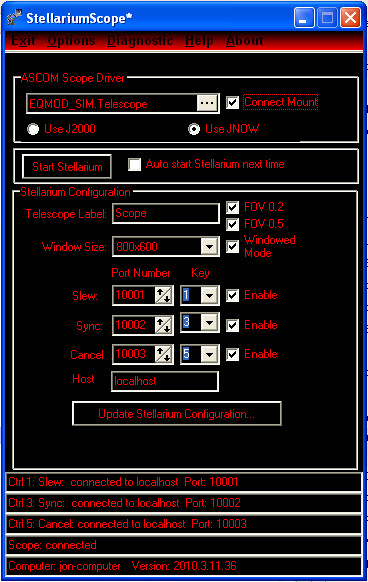
\includegraphics{StellariumScopeFullWindow.jpg}
\end{center}
\label{fig:StellariumScopeFullWindow}
\caption{StellariumScope interface}
\end{figure}

Figure~\ref{fig:StellariumScopeFullWindow} shows the interface and
some of the options.  Use this application (like all software that
controls your mount) with supervision of your mount's movements.

\subsection{Configure StellariumScope}
\label{sec:plugins:StellariumScope:configure}
TODO...
\subsection{Download StellariumScope}
TODO...


\section{Observability Plugin}
\label{sec:plugins.Observability}

TODO...


%%% Local Variables: 
%%% mode: latex
%%% TeX-master: "guide"
%%% End: 

